\documentclass[Main.tex]{subfiles}
\begin{document}
\section{Aanpak}
Omdat de beperkingen van het 'Countdown' probleem niet van toepassing zijn, kunnen een groot deel van de gekende optimalisaties niet gebruikt worden. Als benchmark wordt een brute force algoritme gebruikt. Dit algoritme wordt vervolgens verbeterd door op een effici\"ente manier bepaalde vergelijkingen niet uit te rekenen of in het algemeen te vermijden.
\subsection{Brute Force}
Het brute force algoritme bestaat uit twee stappen. De stappen moeten niet afzonderlijk worden uitgevoerd, maar het levert wel een tijdsvoordeel op indien dit gedaan wordt. De bewerkingsboom kan namelijk eenmalig opgesteld worden en later doorlopen worden.
\subsubsection*{Het opstellen van de bewerkingsboom}
Het opstellen van de bewerkingsboom wordt bereikt door gebruik te maken van de context-vrije grammatica. De root van de bewerkingsboom $E$ wordt uitgebreid aan de hand van de regels van de CFG. De regel $E \rightarrow a,b,\dotsc$) wordt pas in de volgende stap gebruikt. Figuur \ref{fig:bewerkingsboom} toont een voorbeeld van de bewerkingsboom waarbij enkel gebruikt gemaakt wordt van de regels $E \rightarrow E+E$ en $E \rightarrow E \ast E$.
\begin{figure}[!htb]
\centering
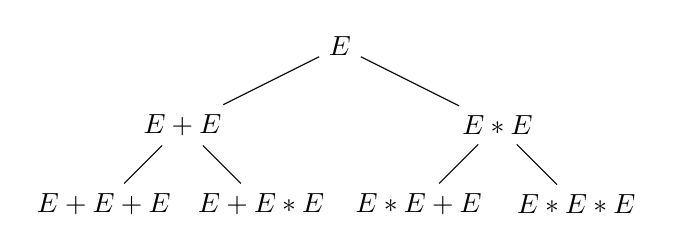
\begin{tikzpicture}[level distance=1cm,
  		level 1/.style={sibling distance=4cm},
  		level 2/.style={sibling distance=2cm}]
  		\node {$E$}
    		child {node {$E+E$}
      		child {node {$E+E+E$}}
      		child {node {$E+E \ast E$}}
    		}
    		child {node {$E \ast E$}
    			child {node {$E \ast E+E$}}
      		child {node {$E \ast E\ast E$}}
    		};
\end{tikzpicture}
\caption{Brute force bewerkingsboom} \label{fig:bewerkingsboom}
\end{figure}
\subsubsection*{Het uitwerken van de vergelijkingen}
In deze stap wordt de regel $E \rightarrow a,b,\dotsc$ gebruikt om elke vergelijking in de bewerkingsboom een waarde te geven. Enkel deze regel wordt gebruikt en voor elke vergelijking wordt elke mogelijkheid afgegaan. Figuur \ref{fig:uitwerkingsboom} toont een gedeeltelijke uitwerking van de bewerkingsboom uit figuur \ref{fig:bewerkingsboom}.
\begin{figure}[!htb]
\centering
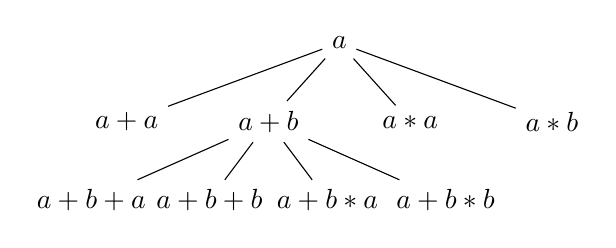
\begin{tikzpicture}[level distance=1cm,
  		level 1/.style={sibling distance=1.8cm},
  		level 2/.style={sibling distance=1.5cm}]
  		\node {$a$}
    		child {node {$a+a$}}
    		child {node {$a+b$}
    		    	child {node {$a+b+a$}}
    			child {node {$a+b+b$}}
    			child {node {$a+b \ast a$}}
    			child {node {$a+b \ast b$}}
    		}
    		child {node {$a \ast a$}}
		child {node {$a \ast b$}};
\end{tikzpicture}
\caption{Uitwerking bewerkingsboom (1 knoop per level)} \label{fig:uitwerkingsboom}
\end{figure}
\subsubsection*{Het resultaat}
Zolang er vergelijkingen worden gezocht waarin geen constanten voorkomen vind dit algoritme in theorie altijd een oplossing. Het is echter wel zeer inefficiënt, zeker naarmate het aantal kolomwaarden\footnote{\label{note:kolomwaarden} De waarden die door de gebruiker worden meegegeven verschillend van de oplossing. In de voorbeelden aangegeven als $a$ en $b$.}
toeneemt.
\subsection{Toevoegen van gewichten}
Het doel van dit algoritme is het vinden van een vergelijking die de gebruiker verlangt. Aangezien een vergelijking zoals $2 \ast x+1$ vaak voorkomt moeten er ook constanten toegelaten worden. Om dit te bereiken manier moet er slechts één wijziging plaatsvinden in het vorige algoritme. Namelijk bij het uitwerken van de vergelijkingen moeten we de regel $E \rightarrow 1,2,\dotsc,9,a,b,\dotsc$ gebruiken in plaats van $E \rightarrow a,b,\dotsc$.
\subsubsection*{Het resultaat}
Het gevolg is dat de uitwerkingstijd van de bewerkingsboom sterk toeneemt. De oplossingsgraad\footnote{\label{note:oplossingsgraad}Het percentage van gevallen waarvoor er een passende oplossing gevonden wordt.}
neemt echter ook sterk toe. De optimale verhouding tussen deze twee wordt bereikt door de keuze van de juiste constanten. Deze keuze zal uit later uit experimenten blijken. Dit algoritme zal gebruikt worden als benchmark.
\subsection{Prunen}
\subsubsection*{Prunen in de bewerkingsboom}
In de bewerkingsboom van het brute force algoritme staan redundante knopen. Hiermee wordt bedoelt: vergelijkingen die altijd hetzelfde resultaat zullen opleveren. Bijvoorbeeld $E \times E+E+E$ en $E+E \times +E$. Echter moet er een verschil gemaakt worden tussen absoluut\footnote{\label{note:absoluut}De knoop en zijn kinderen zijn redundant.} en relatief redundante\footnote{\label{note:relatief}De knoop is redundant maar de kinderen niet.} knopen.%TODO Definitie in probleemstelling, hier of als sterretje beneden? Absoluut = schrappen ook op diepere niveaus, relatief = enkel op huidige niveaus bv ook E+E-E en E-E+E vanwege links toevoegen}%
In het geval van relatief redundante knopen mag de knoop nog niet verwijderd worden wanneer het volgende niveau nog moet berekend worden. In het geval van absoluut redundante knopen mag dit wel. Wanneer de redundante knopen verwijderd worden verkleint de zoekruimte, dit doet de uitwerkingstijd dalen. De oplossingsgraad blijft echter gelijk.
\subsubsection*{Het op voorhand berkenen van de bewerkingsboom}
Het zoeken van redundante knopen vraagt tijd. De bewerkingsboom veranderd niet zolang de CFG niet wijzigt. De mogelijkheid bestaat dus om de boom éénmalig op voorhand op te stellen. Een nadeel aan deze optie is dat het prunen van de uitgewerkte boom (zie verder) tijdrovender wordt. Uit experimenten blijkt dat de tijdswinst van het op voorhand berekenen niet opweegt tegenover het tijdsverlies. Dit komt voornamelijk doordat de tijdswinst op lage niveaus in de berekingsboom ($< 8$) niet groot is en er verwacht wordt dat de gebruiker geen vergelijkingen zoekt van lengte groter dan 6. Het zal later ook blijken dat deze te veel tijd vragen om te berkenen. 
\subsubsection*{Prunen in de uitwerking van de bewerkingsboom}
Ook in de uitwerking van de bewerkingsboom komen er redundante vergelijkingen naar boven. Zo zal de vergelijking $E+E-E$ in sommige gevallen redundant worden. Bijvoorbeeld wanneer ze wordt vervangen door $a+a-a$. Echter is ze niet altijd redundant, ze kan namelijk ook vervangen worden door $a+a-b$. Wanneer er vanuit gegaan wordt dat er constanten in de uitwerking voorkomen onstaan er nog meer redundaties. Zo zal de vergelijking $E+E$ ook terug te vinden zijn als $2*E$. De zoekruimte dus opnieuw verkleint zonder de oplossingsgraad te verlagen.
\subsubsection*{Prunen in realiteit}
Het is mogelijk om alle redundaties te verwijderen zonder de oplossingsgraad\footnotemark[\ref{note:oplossingsgraad}]
te verlagen, dit proces vraagt echter veel rekenwerk en bijgevolg veel tijd. Daarom is er gekozen om sommige redundaties niet te verwijderen (hieronder aangegeven als -), sommige te bewaren (hieronder aangegeven als +) en andere op eenvoudigere wijze uit te werken (hieronder aangegeven als $\ast$). Dit laatste puntje zorgt er echter voor dat er ook niet redundante knopen zullen verloren gaan. Bijvoorbeeld $a+1+1$ kan vervangen worden door $a+2$. Echter vraagt het zoeken van deze redundantie veel tijd. Algemener kan er gezegd worden dat er slechts één losstaande constante mag voorkomen. Het nadeel hiervan is dat het aantal constanten beperkt is, en bijvoorbeeld de vergelijking $a+100$ verloren zal gaan. Maar omdat het doel is te voldoen aan de gebruiker zijn verwachtingen en dus niet alle mogelijkheden te berekenen, is in dit geval de tijdswinst belangrijker dan de lichte daling in oplossingsgraad\footnotemark[\ref{note:oplossingsgraad}].
\subsubsection*{Opsomming prunemogelijkheden}
%TODO tabs voor uitlijning
+ Absoluut redundante knopen in bewerkingsboom\\
	bv. $E \ast E+E+E$ en $E+E \times E+E$\\
+ Onsplitsbare term\footnote{\label{note:onsplitsbaar}Een term van lengte \'e\'en of die enkel bestaat uit bewerkingen met een hogere prioriteit als de optelling. bv $a$ of $a \ast a \div b$}
links $\geq$ dan zijn rechterbuur\\
	bv. $a=2$ en $b=3$ dan mag $b+a$ voorkomen maar $a+b$ niet\\
+ Bewerkingen die bewerkingen ongedaan maken\\
	bv. $a+a-a$ of $a+a/a$ deze laatste kan vervangen worden door $a+1$\\
+ Neutrale constanten\\
	bv. $a \times 1$\\
- Relatief redundante knopen in bewerkingsboom\\
	bv. $E+E \times E$ en $E \times E+E$\\
$\ast$ Toelaten van slechts één losstaand gewicht\\
	bv. $a+1+1$ komt voor als $a+2$\\
$\ast$ Niet toelaten van zelfde onsplistbare term\footnotemark[\ref{note:onsplitsbaar}]\\
	bv. $a+a$ komt voor als $2 \times a$
\subsubsection*{Algoritme}
Algoritme \ref{VindVergelijkingen} bevat de pseudocode van het uiteindelijke resultaat.
%TODO mooier laten uitzien.. niet leesbaar in 1 kolom, miss als bijlage?
\begin{algorithm}[!htb]
\caption{Vind alle mogelijke vergelijkingen}
\label{VindVergelijkingen}
\begin{algorithmic}[1]
\Procedure{Search Equations}{}
\State $\textit{runOutOfTime} \gets \textit{false}$
\State $\textit{currentLevel} \gets \textit{CFG}$.getTerminalRulesAsEquations()
\State $\textit{nextLevel} \gets$new $\textit{List}$
\State $\textit{solutions} \gets$new $\textit{List}$
\While{$\neg\textit{runOutOfTime}$}
	\ForAll{$\textit{currentEq} \gets \textit{currentLevel}$}
		\If{getRunOutOfTime()}
			\State $\textit{runOutOfTime} \gets \textit{true}$
			\State break
		\EndIf
		\ForAll{$\textit{nonTerminalRule} \gets \textit{CFG}$.getNonTerminalRules()}
			\ForAll{$\textit{terminalRule} \gets \textit{CFG}$.getTerminalRules()}
				\State $\textit{newEq} \gets$ expand($\textit{currentEQ, nonTerminalRule, TerminalRule}$)
				\If{isAbsoluteRedundant($\textit{newEq}$)} 
					\State break
				\ElsIf{$\neg$shouldBePruned($\textit{newEq}$)}
					\State $\textit{nextLevel}$.add($\textit{newEq}$)
					\If{$\textit{newEq}$.isGoalReached()} 
						\State $\textit{solutions}$.add($\textit{newEq}$)
					\EndIf
				\EndIf

			\EndFor
		\EndFor
	\EndFor
	\State $\textit{currentLevel} \gets \textit{nextLevel}$
\EndWhile
\EndProcedure
\end{algorithmic}
\end{algorithm}
\end{document}